\documentclass[12pt,a4paper]{article}
\usepackage[
	left 	= 2.54cm,
	right 	= 2.54cm, 
	top 		= 2.54cm,
	bottom 	= 2.54cm,
]{geometry}
\usepackage[utf8]{inputenc}
\usepackage[english]{babel}
\usepackage[OT1]{fontenc}
\usepackage{amsmath}
\usepackage{mathtools}
\usepackage{lscape}
\usepackage{multirow}
\usepackage{booktabs}
\usepackage{graphicx}
\usepackage{caption}
\usepackage{amssymb}

\usepackage[style=apa, backend=biber]{biblatex}
\addbibresource[]{ref.bib}
\renewcommand{\baselinestretch}{1.25} 

\usepackage[hidelinks]{hyperref}
\hypersetup{
	colorlinks = true,
	urlcolor   = blue,
	linkcolor  = black, 
	citecolor  = blue, 
}


\usepackage{fancyhdr}
\pagestyle{fancy}
\lhead{\slshape Unterweger}
\chead{}
\rhead{\slshape \nouppercase{\leftmark}}

\usepackage{titlesec,xcolor}
\titleformat{\section}{\bfseries}{\thesection}{0.5em}{}
\titlespacing{\section}{0pt}{3ex plus 1ex minus 0.2ex}{10pt}
\setlength{\headheight}{14.49998pt}

\usepackage{titlesec,xcolor}
\titleformat{\subsection}{\bfseries}{\thesubsection}{0.5em}{}
\titlespacing{\subsection}{0pt}{3ex plus 1ex minus 0.2ex}{10pt}
\setlength{\headheight}{14.49998pt}

%% Command Overrides
\newcommand{\norm}[1]{\left\lVert#1\right\rVert}
\DeclareMathOperator*{\argmax}{arg\,max}
\DeclareMathOperator*{\argmin}{arg\,min}
\newcommand{\MC}{\textbf{(Missing Citation)}} %Command to signal missing citations



%------------------------------------------------------------------%

\author{Lucas Paul Unterweger}
\title{On the Duality of Frequentist Point Estimates and Bayesian Shrinkage Priors: An Extension based on the Triple-Gamma-Prior}


\begin{document}

\begin{titlepage}
\center
\vfill

\includegraphics[scale=0.1]{WU.png}
\vfill
\begin{tabular}[t]{lc}
Student-ID:  & 11913169 \\
Degree Program: & 
Master of Science in Economics (Science Track) \\
Examiner: & Peter Knaus, PhD \\
Submission date: & TBA \\
\end{tabular}
\vfill
{\large \textbf{Triple-Gamma-Regularization} \textit{or}\\ \textbf{On the Duality of Frequentist Point Estimates and Bayesian Shrinkage Priors}\\
\normalsize \textit{An Extension based on the Triple-Gamma-Prior}}
\vfill
by\\ \vspace{3mm}
{\Large Lucas Unterweger \href{https://github.com/therealLucasPaul}{
\includegraphics[scale=0.01]{GitHub.png}}}\\
(Student-ID: 11913169)\\
\vfill

\thispagestyle{empty}
\pagebreak
\end{titlepage}
\newcounter{savepage}
\pagenumbering{roman}
\thispagestyle{empty}

\begin{abstract}
Lorem ipsum...
\end{abstract}

\clearpage
\thispagestyle{plain}
\tableofcontents
\pagebreak
\setcounter{savepage}{\arabic{page}}
\pagenumbering{arabic}

\pagebreak
%----- Introduction -----
\section{Introduction}
Willam of Ockham, born in Ockham, Surrey, probably lived between 1287 and 1348 and is nowadays recognized as a pre-eminent philosopher of the middle ages. Although     his name itself is no common knowledge, a principle carrying his name is: \textit{Ockham's Razor}. Interestingly, the main formulation of the principle (\textit{Entia non sunt multiplicanda praeter necessitatem} [plurality should not be posited without necessity]) can not be traced back to Ockham directly, but variations of it can be found in Ockham's writings. Since then nonetheless, the principle has long been used by statisticians and other researchers as a a scientific credo to capture the notion that "the simpler of two explanations is to be preferred" \parencite{Lazar2010}.  
%----- Literature Review -----


\section{Literature Review}
\subsection{Bayesian View}
\subsection{Frequentist View}


%----- Theoretical Section
\section{Theoretical Section}\label{sec:theorysuper}
\subsection{Model Complexity}
Overfitting is a problem. Especially when dimensionality issues arise. For example, 50 observations and 20 features. Model will perform well/almost perfect on training data, but will do terrible on training data.\\
\subsection{Under- and Overfitting}

General problem: Fit vs. Complexity. What to choose and where is the optimal balance?

Solutions (find source, seen in LMU course): (1) More data (Not always feasible) (2) Better data (Same issue) (3) Reduce Model Complexity (Regularization) (4) Less aggressive optimization (Maybe short review; Idea: Stop optimization when generalization error degrades)

\subsubsection{Regularization}
Ad Solution (3) because it is relatively easy to implement: Simple approach => Start with simplest model and iteratively add one feature OR iteratively get rid of feature by feature. (Problem: Very arbitrary and hard to reasonably do) Thus, adjust risk function minimization. Important: Regularization adjusts generalization error, not training error!

Short break: Talk about Taxonomy by Kukacka et al 2017 on the differing use of the term "regularization" 

What is needed: 
\[
R_{reg}(\beta) = R_{emp}(\beta)+ \lambda \cdot J(\beta)
\]
where $R_{emp}(\beta) = \sum_i^n L(y_i, f(x_i, \beta))$. Note: Regularization term does not depend on data, just on parametrization. $\lambda$ controls the strength of regularization. Thus, $\lambda = 0$ means simple MSE optimization and $\lambda \to \infty$ chooses simplest model. As $\lambda$ is set manually, this also bears some problems. However, typical solution is cross-validation. 
\subsubsection{Short Deviation to Bayesian Shrinkage Priors}

\subsection{Duality of the Ridge Regression}

\subsection{Triple-Gamma-Prior by \textcite{TGP2020}}

%----- Model Setup and Derivation
\newpage
\section{Model Setup and Derivation}
Coming to the theoretical framework of the \textit{triple-gamma-regularization}, let's assume we have a response variable $y$ and $p$ predictors along with $n$ data points. More formally, let $y=[y_1  \quad y_2 \cdots y_n]^T$ and $x_i = [x_{i1} \quad x_{i2} \cdots x_{in}]^T$ with $\forall i\in \{1,...,n\}: y_i, x_i \in \mathbb{R}$. Here, $x_i$ is the $i$-th predictor, thus resulting in the design matrix $X = [x_1 \quad x_2 \cdots x_p]$. \\

Starting from the Bayesian framework, the standard linear regression model is given by
\[
y_i = x_i^T\cdot \beta + \varepsilon_i \quad i\in \{1,...,n\} 
\]
with the assumed distribution of $\varepsilon_i \sim N(0,\sigma^2)$. Thus it follows that $y\sim N_n(X\beta,\sigma^2I)$. The posterior distribution of the parameter vector $\beta$, according to Bayes' Rule, is then proportional to the product of the likelihood of the data and the prior distribution, which can be seen in equation \ref{eq:bayes}.
\begin{equation}\label{eq:bayes}
p(\beta|y, X, \sigma^2) \propto \mathcal{L}(y|\beta, \sigma^2, X)\times p(\beta)
\end{equation}	

As stated above, each data point $y_i$ is assumed to be identically and independently drawn from a normal distribution with mean $X\beta$ and variance $\sigma_i^2$, thus:
\begin{align}
\mathcal{L}(\mathbf{y}|\beta, \sigma^2, X) 	&= \prod_i^n p(y_i|\beta, \sigma^2, X_i) \nonumber\\
						&= \prod_i^n \frac{1}{\sqrt{2\pi\sigma^2}} \exp\left(-\frac{1}{2}\left(\frac{x_i-\mu}{\sigma}\right)^2\right) \nonumber\\
						&= \frac{1}{(2\pi\sigma^2)^{n/2}}\exp\left(-\frac{1}{2\sigma^2}(\mathbf{y}-\mathbf{X}\beta)^\top(\mathbf{y}-\mathbf{X}\beta)\right) \label{eq:likelihood}
\end{align}

The log of the likelihood function is then given by 
\begin{align*}
\log \mathcal{L}( \mathbf{y} |\beta, \sigma^2 , \mathbf{X}) &= \log \left( \frac{1}{(2\pi\sigma^2)^{n/2}} \exp\left(-\frac{1}{2\sigma^2} (\mathbf{y} - \mathbf{X}\beta)^\top (\mathbf{y} - \mathbf{X}\beta)\right) \right) \\
&= \log \left( \frac{1}{(2\pi\sigma^2)^{n/2}} \right) + \log \exp\left(-\frac{1}{2\sigma^2} (\mathbf{y} - \mathbf{X}\beta)^\top (\mathbf{y} - \mathbf{X}\beta)\right) \\
&= -\frac{n}{2} \log(2\pi\sigma^2) - \frac{1}{2\sigma^2} (\mathbf{y} - \mathbf{X}\beta)^\top (\mathbf{y} - \mathbf{X}\beta)\\
&\propto - \frac{1}{2\sigma^2} (\mathbf{y} - \mathbf{X}\beta)^\top (\mathbf{y} - \mathbf{X}\beta) = - \frac{1}{2\sigma^2}\norm{\mathbf{y} - \mathbf{X}\beta}_2^2\\
\end{align*}

The marginal prior distribution for the parameter vector $\beta$ stems from the Triple-Gamma-Prior constructed in \textcite{TGP2020} given in Theorem 1 (a) and is given by
\begin{align*}
p(\sqrt{\beta_j}|\phi^\xi, a^\xi, c^\xi) &= \frac{\Gamma(c^\xi + \frac{1}{2})}{\sqrt{2\pi \phi^\xi}\cdot B(a^\xi, c^\xi)}\cdot U\left(c^\xi + \frac{1}{2}, \frac{3}{2}-a^\xi, \frac{\beta_j}{2\phi^\xi}\right)\\
&\propto U\left(c^\xi + \frac{1}{2}, \frac{3}{2}-a^\xi, \frac{\beta_j}{2\phi^\xi}\right)
\end{align*}
Here, $U(a,b,z)$ refers the confluent hyper-geometric function of the second kind which was introduced by \textcite{Tricomi1947}. As this prior is specified for the parameter $\sqrt{\beta_j}$, we transform the prior by squaring the parameter to gain
\begin{align*}
p(\beta_j|\phi^\xi, a^\xi, c^\xi) &\propto U\left(c^\xi + \frac{1}{2}, \frac{3}{2}-a^\xi, \frac{\beta_j^2}{2\phi^\xi}\right)
\end{align*}
Now, assuming that the parameters are independent a priori, the prior distribution is given by
\begin{align}
p(\beta) 	&= \prod_j^p p(\beta_j) \nonumber\\
			&= \prod_j^p p(\beta_j|\phi^\xi, a^\xi, c^\xi) \nonumber\\
			&\propto \prod_j^p U\left(c^\xi + \frac{1}{2}, \frac{3}{2}-a^\xi, \frac{\beta_j^2}{2\phi^\xi}\right) \nonumber\\
			&= \prod_j^p \frac{1}{\Gamma(c^\xi + \frac{1}{2})}\int_0^\infty e^{-(\frac{\beta_j^2}{2\phi^\xi})t}t^{c^\xi + \frac{1}{2}-1}(1+t)^{\frac{3}{2}-a^\xi-c^\xi + \frac{1}{2}-1}dt \nonumber\\
			&\propto \prod_j^p \int_0^\infty \exp\left(-\frac{\beta_j^2}{2\phi^\xi}t\right)t^{c^\xi - \frac{1}{2}}(1+t)^{1-a^\xi-c^\xi} dt \label{eq:prior}
\end{align}

Here, in line 1 the assumption of independence between the parameters has been used to describe the distribution of the parameter vector as the product of its individual parameter distributions. In line 2, the marginal prior from \textcite{TGP2020} has been used as the prior distribution for each individual parameter $\beta_j$. In line 3, scaling parameters have been removed by using the proportionality assumption. The last two lines of the derivation insert the integral representation of the confluent hyper-geometric function of the second kind, $U(a,b,z)$, which is valid in the case of a positive real part for the first parameter ($\mathfrak{Re}(a) > 0$) and again apply proportionality.\\

Taking the $\log$ of the prior distribution and using the properties of the logarithmic function yields the general result
\[
\log(p(\beta))=\log(\prod_j^p p(\beta_j|\phi^\xi, a^\xi, c^\xi))=\sum_j^p \log(p(\beta_j|\phi^\xi, a^\xi, c^\xi))
\]

A common approach to estimation in regularization settings is the \textit{maximum a posteriori probability (MAP)} estimator \MC ,which is defined as
\[
\hat{\beta}_{MAP}(x) = \underset{\beta \in \mathbb{R}^p}{\argmax}\left\{f(x|\beta)g(\beta)\right\}
\]
where $f(x|\beta)$ describes the the probability density function of a variable $x$, which is parametrized by the parameter vector $\beta$. The second function $g(\beta)$ incorporates our prior information about the parameter vector $\beta$ into the optimization problem.\\  

Returning to our specific problem at hand, the posterior distribution of our parameter vector $\mathbf{\beta}$ can be retrieved by applying Bayes' theorem and the previously gained results in equations \ref{eq:prior} and \ref{eq:likelihood}. Thus, the posterior distribution of the parameter vector $\beta$ is proportional to
\begin{align}
p(\beta|y, X, \sigma^2) 	&\propto p(y|X,\beta,\sigma)\times p(\beta) \nonumber\\
						&\propto \frac{1}{(2\pi\sigma^2)^{n/2}}e^{-\frac{1}{2\sigma^2}(y-X\beta)^T(y-X\beta)} \times \prod_j^p U\left(c^\xi + \frac{1}{2}, \frac{3}{2}-a^\xi, \frac{\beta_j^2}{2\phi^\xi}\right)\label{eq:posterior}
\end{align} 

Making use of the monotonicity of the logarithmic function and seeing that it is easier to optimize the log-posterior, Taking the log of the posterior probability distribution, we take the log of result \ref{eq:posterior}. 
\begin{align}
\log(\beta| X, y, \sigma^2) 	&= \log\left(\frac{1}{(2\pi\sigma^2)^{n/2}}\right) - \frac{1}{2\sigma^2}\norm{\mathbf{y} - \mathbf{X}\beta}_2^2 + \log\left(\prod_j^p U\left(c^\xi + \frac{1}{2}, \frac{3}{2}-a^\xi, \frac{\beta_j^2}{2\phi^\xi}\right)\right)\nonumber\\
							&= \log\left(\frac{1}{(2\pi\sigma^2)^{n/2}}\right) - \frac{1}{2\sigma^2}\norm{\mathbf{y} - \mathbf{X}\beta^2}_2^2 + \sum_j^p \log\left(U\left(c^\xi + \frac{1}{2}, \frac{3}{2}-a^\xi, \frac{\beta_j}{2\phi^\xi}\right)\right)\nonumber\\
							&\propto -\frac{1}{2\sigma^2}\norm{\mathbf{y} - \mathbf{X}\beta}_2^2 + \sum_j^p \log\left(U\left(c^\xi + \frac{1}{2}, \frac{3}{2}-a^\xi, \frac{\beta_j^2}{2\phi^\xi}\right)\right)\nonumber\\
\end{align}

To align with the general specification structure of regularization problems, which can be seen from equation \textbf{missEQ}, a parameter $\lambda$ will be multiplicatively added in front of the penalty term, which makes it possible to adjust the strength of the influence that the penalty has on the chosen parameters. By minimizing the negative log-posterior adjusted with $\lambda$, we can retrieve the \textit{maximum a posteriori probability (MAP)} estimator using \textbf{Triple-Gamma-Regularization}:
\begin{equation}\label{eq:tgr}
\hat{\beta}_{MAP} = \underset{\beta \in \mathbb{R}^p}{\argmin} \left(\frac{1}{2\sigma^2}\norm{\mathbf{y} - \mathbf{X}\beta}_2^2 + \lambda \sum_j^p -\log\left(U\left(c^\xi + \frac{1}{2}, \frac{3}{2}-a^\xi, \frac{\beta_j^2}{2\phi^\xi}\right)\right)\right) 
\end{equation}

\newpage
\subsection{Varying the Hyperparameters}
After closer inspection of equation \ref{eq:tgr}, it can easily be seen that this resembles the general penalized regression already seen in \textcite{ESLpage398} and in section \ref{sec:theorysuper} as $R(\beta) + \lambda\cdot J(\beta)$. The first term, alos called the empirical loss in machine learning literature, is the widely known residual sum of squares:
\[
R(\beta)=\frac{1}{2\sigma^2}\norm{\mathbf{y} - \mathbf{X}\beta}_2^2
\] 
The second part of the optimization problem can be viewed as a penalty imposed on the total risk based on the size of the estimates:
\[
J(\beta) = \sum_j^p -\log\left(U\left(c^\xi + \frac{1}{2}, \frac{3}{2}-a^\xi, \frac{\beta_j^2}{2\phi^\xi}\right)\right)
\]
In contrast to the \textit{LASSO} penalty, which uses the the absolute value of the coefficient, or the \textit{Ridge} penalty, which uses the square of the estimate, this penalty derived from \textcite{TGP2020} is based on the $\log$ of the confluent hyper-geometric of the second kind. Notably, this penalty term has three additional hyper-parameters: $c^\xi$, $a^\xi$ and $\kappa$ as $\phi^\xi = (2c^\xi)/(\kappa^2_B a^\xi)$.

\begin{figure}[!h]
\centering
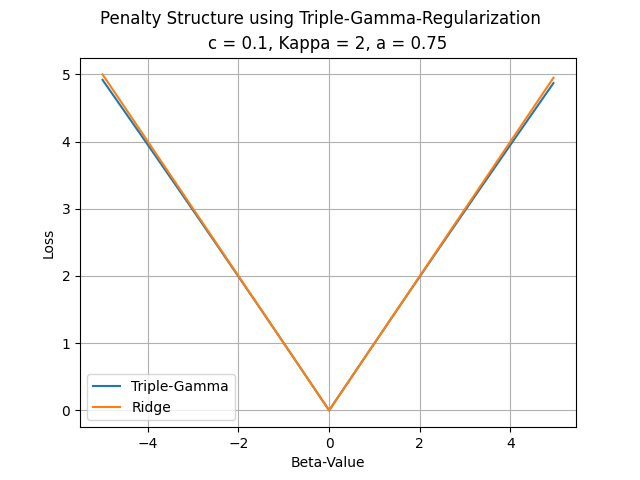
\includegraphics[scale=0.75]{../02_simulation/021_simulation_figures/simpleTGpenalty.png}
\caption{Basic Representation of the Triple-Gamma-Penalty using Hyperparameters $c^\xi = 0.1, \kappa_B = 2, a^\xi = 0.75$ compared to \textit{LASSO} and \textit{Ridge} Penalties}
\label{fig:basicTGPen}
\end{figure}

\begin{figure}[!h]
\centering
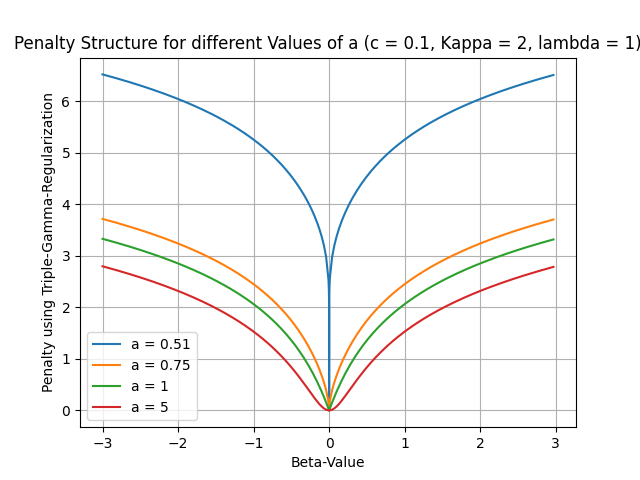
\includegraphics[scale=0.75]{../02_simulation/021_simulation_figures/TGPenalty_ChangeInA.png}
\caption{Triple-Gamma-Penalty using different values of $a^\xi$}
\label{fig:basicTGPen}
\end{figure}

\begin{figure}[!h]
\centering
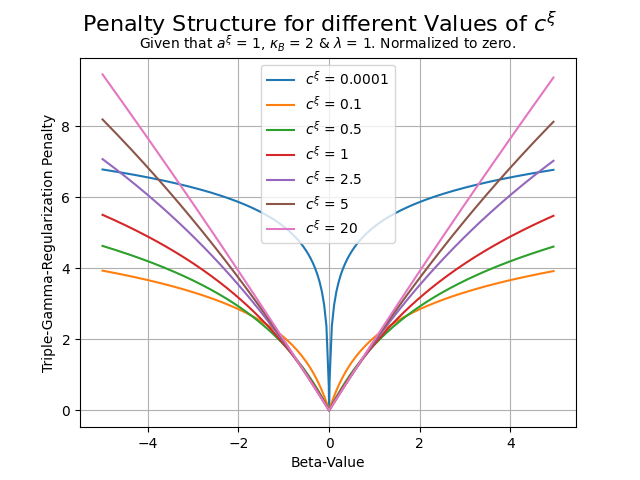
\includegraphics[scale=0.75]{../02_simulation/021_simulation_figures/TGPenalty_ChangeInC.png}
\caption{Triple-Gamma-Penalty using different values of $c^\xi$}
\label{fig:basicTGPen}
\end{figure}

\begin{figure}[!h]
\centering
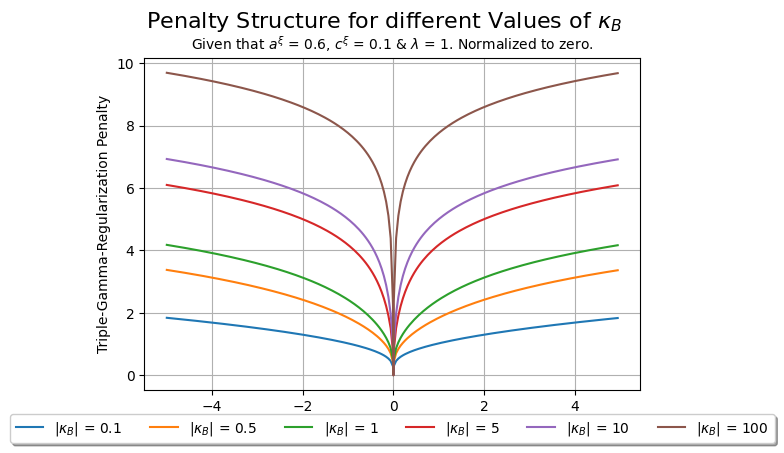
\includegraphics[scale=0.75]{../02_simulation/021_simulation_figures/TGPenalty_ChangeInKappa.png}
\caption{Triple-Gamma-Penalty using different values of $\kappa_B$}
\label{fig:basicTGPen}
\end{figure}

\subsection{Restricted Strong Convexity (RSC) of the Triple-Gamma-Regularization}

\subsection{Alternative Specification (with +1 to mimic artan)}

\subsection{Approaches to Estimation}

%----- Simulation Section
\section{Simulation Section}
Use the earlier derivation, code up the functions and simulate data to check behaviour for different datasets. Compare to base OLS, Ridge and Lasso Regression?
\subsection{Computational Performance}
Talking about Gradient Descent Methods in more depth. Why Gradient Clipping. Maybe more modern estimation techniques? 
\subsection{Implementation as Python Library}

How to use it. 
Explanation of Functions. Input - Output Tables

%----- Small Applied Section
\section{Small Applied Section}
Here I am planning to apply the TGP using Peter's Bayesian Package and the self coded frequentist code on a small dataset.
\section{Conclusion}
\section{Possible Extensions and Criticism}
\section{References}

\pagebreak
\pagenumbering{roman}
\setcounter{page}{\thesavepage}
\pagestyle{plain}
\addcontentsline{toc}{section}{References}
%\bibliographystyle{apalike}
%\bibliography{ref.bib}
\printbibliography[]
\clearpage
\appendix
\end{document}
